\section{Studierendenpflichten}
\textbf{Sodele!}\\
Dies hier ist nun der Moralteil. Wie immer im Leben gibt es diverse persönliche Pflichten, die euch das Überleben sichern und einige moralische Pflichten, die euch zu einem moralisch starken Menschen machen\ldots Die ersten dieser Pflichten wurden euch ja schon präsentiert und lauten -- noch mal zusammengefasst -- Arbeiten, Arbeiten und zwischendurch aufpassen, dass man die richtigen Fächer belegt\ldots\\
Viele denken, dass damit sozusagen ihre Studierendenpflicht endet. Im Grunde genommen stimmt das vielleicht auch offiziell, wenn da nicht noch die \enquote{politischen Pflichten} der Studierenden wären. Es war und ist nicht eure Pflicht, auf die Stra\ss en zu rennen und Autos anzuzünden, weil ihr die Hochschulpolitik des Landes schei\ss e findet, was ja verständlich ist, wenn man mal locker 500 \euro{} weniger im Semester haben könnte; aber, euch über die momentane Situation zu informieren. Solltet ihr dies vorhaben, gibt es drei Anlaufstellen:
\begin{enumerate}
   \item den Allgemeinen Studierendenausschuss (AStA)
   \item die Fachschaft bzw. den Fachschaftsrat
   \item das Internet
\end{enumerate}
Natürlich muss dieses Heft auch Schleichwerbung enthalten, weswegen ich Nr. 2 empfehle.\\
Am Ende des Wintersemesters finden jedes Jahr Wahlen zum Studierendenparlament, Fachbereichs-- und Fachschaftsrat sowie zum Senat statt.\\
Du solltest von Anfang an deine Stimme abgeben, denn dies ist wichtig. Damit stärkt ihr die Position eurer Vertreter, die sich in vielen verschiedenen Belangen für euch einsetzen (zum Beispiel die Verhandlungen über das Semesterticket führen).
Daher lautet unser Aufruf:\\
\textbf{Geht wählen}!!!\\
Es ist ein kleines Kreuz für euch, aber ein gro\ss es für die Studierendenschaft.\\
Wer sich über das Kreuzchen machen hinaus, wenn auch vielleicht nicht gerade gleich im ersten Semester,hochschulpolitisch engagieren und mitreden möchte, hat dazu eine Vielzahl an Möglichkeiten und sollte diese auch wahrnehmen: Am einfachsten ist es sicherlich, aktiv in der Fachschaft, im Fachschafts-- oder Fachbereichsrat mitzuarbeiten. Hier kann man zwar nur wenig Einfluss auf die Grundsatzentscheidungen der gesamten Universität nehmen, aber man kann sich für sinnvolle Veränderungen an unserem Fachbereich Physik stark machen.
\von{Fritz}
\begin{center}
  	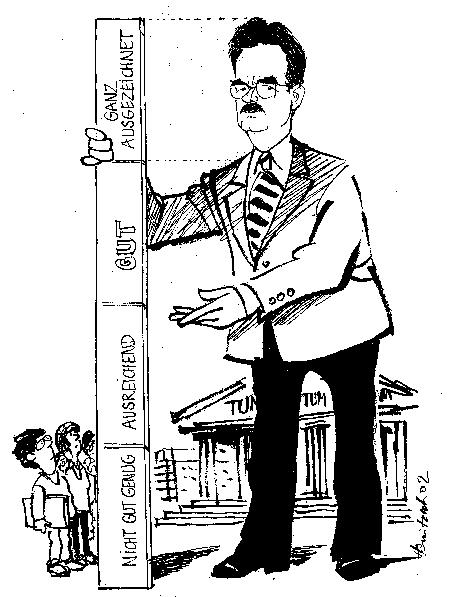
\includegraphics[width=0.8\textwidth]{\imgdir/steinberg.jpg}
\end{center}